%%%%%%%%%%%%%%%%%%%%%%%%%%%%%%%%%%%%%%%%%%%%%%%%%%%%%%%%%%%

%% document class
\documentclass[a4paper]{article}

%% packages
%% packages

\usepackage{blindtext} % needed for creating dummy text passages
\usepackage{amsmath} % needed for command eqref
\usepackage{amssymb} % needed for math fonts

\usepackage{pifont}% For ticks and crosses as defined in the newcommands below. More info at http://ctan.org/pkg/pifont
\newcommand{\cmark}{\ding{51}}%
\newcommand{\xmark}{\ding{55}}%

%%%%%%%%%%%%%%%%%%%%%%%%%%%%%%%%%%%%%%%%%%%%%%%%%%%%%%%%%%%
\usepackage[
	colorlinks=true
	,breaklinks %in case some labels are too long and may span several pages, e.g. in List of Figures, etc.
	]{hyperref} % needed for creating hyperlinks in the document, the option colorlinks=true gets rid of the awful boxes, breaklinks breaks long links (list of figures), and ngerman sets everything for german as default hyperlinks language
\usepackage[hyphenbreaks]{breakurl} % ben�tigt f�r das Brechen von URLs in Literaturreferenzen, hyphenbreaks auch bei links, die �ber eine Seite gehen (mit hyphenation).

\usepackage{xcolor}
\definecolor{c1}{rgb}{0,0,1} % blue
\definecolor{c2}{rgb}{0,0.3,0.9} % light blue
\definecolor{c3}{rgb}{0.3,0,0.9} % red blue
\hypersetup{
    linkcolor={c1}, % internal links
    citecolor={c2}, % citations
    urlcolor={c3} % external links/urls
}

%\usepackage{cite} % needed for cite
\usepackage[round,authoryear]{natbib} % needed for cite and abbrvnat bibliography style
\usepackage[nottoc]{tocbibind} % needed for displaying table of contents, bibliography, index and other in the table of contents. 'nottoc' is to exclude the phreases "table of contents" from the table of contents.
%%%%%%%%%%%%%%%%%%%%%%%%%%%%%%%%%%%%%%%%%%%%%%%%%%%%%%%%%%%

\usepackage{graphicx} % needed for \includegraphics
\usepackage{subcaption} % for creating subfigures (side-by-side) and captioning them
\usepackage{float}	% to insert tables at precise position of code with [H] specifier.
\usepackage{longtable} % needed for long tables over pages
\usepackage{bigstrut} % needed for the command \bigstrut
\usepackage{enumerate} % needed for some options in enumerate
\usepackage{todonotes} % needed for todos
\usepackage{makeidx} % needed for creating an index
\makeindex
\usepackage{color}
\usepackage{siunitx} % for commonly used SI unit symbols with command SI{value}{unit}, SIrage, etc.
\usepackage{pdfpages} % for inserting pdf pages with command \includepdf{<filename>}
\usepackage{listings} % to insert source code of any programming language
\lstset{
basicstyle=\footnotesize,
frame=single,
numbers=left,
keepspaces=true,
breaklines=true,
commentstyle=\color[rgb]{0,0.6,0},
keywordstyle=\color{blue},
stringstyle=\color[rgb]{0.8,0,0}
}
%%% packages

\usepackage{blindtext} % needed for creating dummy text passages
\usepackage{amsmath} % needed for command eqref
\usepackage{amssymb} % needed for math fonts

\usepackage{pifont}% For ticks and crosses as defined in the newcommands below. More info at http://ctan.org/pkg/pifont
\newcommand{\cmark}{\ding{51}}%
\newcommand{\xmark}{\ding{55}}%

%%%%%%%%%%%%%%%%%%%%%%%%%%%%%%%%%%%%%%%%%%%%%%%%%%%%%%%%%%%
\usepackage[
	colorlinks=false,	% color links
	breaklinks %in case some labels are too long and may span several pages, e.g. in List of Figures, etc.
	]{hyperref} % needed for creating hyperlinks in the document, the option colorlinks=true gets rid of the awful boxes, breaklinks breaks long links (list of figures), and ngerman sets everything for german as default hyperlinks language
\usepackage[hyphenbreaks]{breakurl} % ben�tigt f�r das Brechen von URLs in Literaturreferenzen, hyphenbreaks auch bei links, die �ber eine Seite gehen (mit hyphenation).

\usepackage{xcolor}
\definecolor{c1}{rgb}{0,0,1} % blue
\definecolor{c2}{rgb}{0,0.3,0.9} % light blue
\definecolor{c3}{rgb}{0.3,0,0.9} % red blue
%\hypersetup{
%    linkcolor={c1}, % internal links
%    citecolor={c2}, % citations
%    urlcolor={c3} % external links/urls
%}

%\usepackage{cite} % needed for cite
\usepackage[round,authoryear]{natbib} % needed for cite and abbrvnat bibliography style
\usepackage[nottoc]{tocbibind} % needed for displaying table of contents, bibliography, index and other in the table of contents. 'nottoc' is to exclude the phreases "table of contents" from the table of contents.
%%%%%%%%%%%%%%%%%%%%%%%%%%%%%%%%%%%%%%%%%%%%%%%%%%%%%%%%%%%

\usepackage{graphicx} % needed for \includegraphics
\usepackage{subcaption} % for creating subfigures (side-by-side) and captioning them
\usepackage{float}	% to insert tables at precise position of code with [H] specifier.
\usepackage{longtable} % needed for long tables over pages
\usepackage{bigstrut} % needed for the command \bigstrut
\usepackage{enumerate} % needed for some options in enumerate
\usepackage{todonotes} % needed for todos
\usepackage{makeidx} % needed for creating an index
\makeindex
\usepackage{color}
\usepackage{siunitx} % for commonly used SI unit symbols with command SI{value}{unit}, SIrage, etc.
\usepackage{pdfpages} % for inserting pdf pages with command \includepdf{<filename>}
\usepackage{listings} % to insert source code of any programming language
\lstset{
basicstyle=\footnotesize,
frame=single,
numbers=left,
keepspaces=true,
breaklines=true,
%commentstyle=\color[rgb]{0,0.6,0},
%keywordstyle=\color{blue},
%stringstyle=\color[rgb]{0.8,0,0}
}

%% page settings
%% page settings

\usepackage[top=1in, bottom=1in, left=1in, right=1in]{geometry} % needed for page border settings
\parindent=0cm % for space of first line of new text block
\parskip=5pt % for space between paragraphs
\sloppy % for writing with hyphenless justification (tries to)
\hyphenation{} % use hyphenation of tolerance parameters, http://www.jr-x.de/publikationen/latex/tipps/zeilenumbruch.html
\hyphenpenalty=10000
%\exhyphenpenalty=10000
%\usepackage{fancyhdr} % needed for head and foot options
%\linespread{1.15} % needed for inter-line spacing
%\pagenumbering{gobble} % to disable page numbering

%% own commands
%% my macros

%% Text fomats
\newcommand{\tbi}[1]{\textbf{\textit{#1}}}
\newcommand{\redfont}[1]{\textcolor{red}{#1}}

%% Math fonts
\newcommand{\bbA}{\mathbb{A}}
\newcommand{\bbB}{\mathbb{B}}
\newcommand{\bbC}{\mathbb{C}}
\newcommand{\bbD}{\mathbb{D}}
\newcommand{\bbE}{\mathbb{E}}
\newcommand{\bbF}{\mathbb{F}}
\newcommand{\bbG}{\mathbb{G}}
\newcommand{\bbH}{\mathbb{H}}
\newcommand{\bbI}{\mathbb{I}}
\newcommand{\bbJ}{\mathbb{J}}
\newcommand{\bbK}{\mathbb{K}}
\newcommand{\bbL}{\mathbb{L}}
\newcommand{\bbM}{\mathbb{M}}
\newcommand{\bbN}{\mathbb{N}}
\newcommand{\bbO}{\mathbb{O}}
\newcommand{\bbP}{\mathbb{P}}
\newcommand{\bbQ}{\mathbb{Q}}
\newcommand{\bbR}{\mathbb{R}}
\newcommand{\bbS}{\mathbb{S}}
\newcommand{\bbT}{\mathbb{T}}
\newcommand{\bbU}{\mathbb{U}}
\newcommand{\bbV}{\mathbb{V}}
\newcommand{\bbW}{\mathbb{W}}
\newcommand{\bbX}{\mathbb{X}}
\newcommand{\bbY}{\mathbb{Y}}
\newcommand{\bbZ}{\mathbb{Z}}

%% SI units
\newcommand{\degC}[1]{\SI{#1}{\degreeCelsius}}

%%%%%%%%%%%%%%%%%%%%%%%%%%%%%%%%%%%%%%%%%%%%%%%%%%%%%%%%%%%

\begin{document}

%\pagestyle{empty}
%\title{ME3291 Homework Assignment}
%\author{Chua Ping Chan}
%\date{}
%\maketitle

%%%%%%%%%%%%%%%%%%%%%%%%%%%%%%%%%%%%%%%%%
% University Assignment Title Page 
% LaTeX Template
% Version 1.0 (27/12/12)
%
% This template has been downloaded from:
% http://www.LaTeXTemplates.com
%
% Original author:
% WikiBooks (http://en.wikibooks.org/wiki/LaTeX/Title_Creation)
%
% License:
% CC BY-NC-SA 3.0 (http://creativecommons.org/licenses/by-nc-sa/3.0/)
% 
% Instructions for using this template:
% This title page is capable of being compiled as is. This is not useful for 
% including it in another document. To do this, you have two options: 
%
% 1) Copy/paste everything between \begin{document} and \end{document} 
% starting at \begin{titlepage} and paste this into another LaTeX file where you 
% want your title page.
% OR
% 2) Remove everything outside the \begin{titlepage} and \end{titlepage} and 
% move this file to the same directory as the LaTeX file you wish to add it to. 
% Then add %%%%%%%%%%%%%%%%%%%%%%%%%%%%%%%%%%%%%%%%%
% University Assignment Title Page 
% LaTeX Template
% Version 1.0 (27/12/12)
%
% This template has been downloaded from:
% http://www.LaTeXTemplates.com
%
% Original author:
% WikiBooks (http://en.wikibooks.org/wiki/LaTeX/Title_Creation)
%
% License:
% CC BY-NC-SA 3.0 (http://creativecommons.org/licenses/by-nc-sa/3.0/)
% 
% Instructions for using this template:
% This title page is capable of being compiled as is. This is not useful for 
% including it in another document. To do this, you have two options: 
%
% 1) Copy/paste everything between \begin{document} and \end{document} 
% starting at \begin{titlepage} and paste this into another LaTeX file where you 
% want your title page.
% OR
% 2) Remove everything outside the \begin{titlepage} and \end{titlepage} and 
% move this file to the same directory as the LaTeX file you wish to add it to. 
% Then add %%%%%%%%%%%%%%%%%%%%%%%%%%%%%%%%%%%%%%%%%
% University Assignment Title Page 
% LaTeX Template
% Version 1.0 (27/12/12)
%
% This template has been downloaded from:
% http://www.LaTeXTemplates.com
%
% Original author:
% WikiBooks (http://en.wikibooks.org/wiki/LaTeX/Title_Creation)
%
% License:
% CC BY-NC-SA 3.0 (http://creativecommons.org/licenses/by-nc-sa/3.0/)
% 
% Instructions for using this template:
% This title page is capable of being compiled as is. This is not useful for 
% including it in another document. To do this, you have two options: 
%
% 1) Copy/paste everything between \begin{document} and \end{document} 
% starting at \begin{titlepage} and paste this into another LaTeX file where you 
% want your title page.
% OR
% 2) Remove everything outside the \begin{titlepage} and \end{titlepage} and 
% move this file to the same directory as the LaTeX file you wish to add it to. 
% Then add \input{./title_page_1.tex} to your LaTeX file where you want your
% title page.
%
%%%%%%%%%%%%%%%%%%%%%%%%%%%%%%%%%%%%%%%%%

%----------------------------------------------------------------------------------------
%	PACKAGES AND OTHER DOCUMENT CONFIGURATIONS
%----------------------------------------------------------------------------------------

%\documentclass[12pt]{article}
%
%\begin{document}

\begin{titlepage}

\newcommand{\HRule}{\rule{\linewidth}{0.5mm}} % Defines a new command for the horizontal lines, change thickness here

\center % Center everything on the page
 
%----------------------------------------------------------------------------------------
%	HEADING SECTIONS
%----------------------------------------------------------------------------------------
\quad\\[2cm]
\textsc{\LARGE National University of Singapore}\\[1.5cm] % Name of your university/college
\textsc{\Large ME3291 Numerical Methods in Engineering}\\[0.5cm] % Major heading such as course name
%\textsc{\large Homework Assignment}\\[0.5cm] % Minor heading such as course title

%----------------------------------------------------------------------------------------
%	TITLE SECTION
%----------------------------------------------------------------------------------------

\HRule \\[0.6cm]
{ \huge \bfseries Numerical Methods:\\[0.5cm]
Temperature Distribution (Plate)}\\[0.4cm] % Title of your document
\HRule \\[2cm]
 
%----------------------------------------------------------------------------------------
%	AUTHOR SECTION
%----------------------------------------------------------------------------------------

%\begin{minipage}{0.4\textwidth}
%\begin{flushleft} \large
%\emph{Author:}\\
%\textsc{Chua Ping Chan} % Your name
%\end{flushleft}
%\end{minipage}
%~
%\begin{minipage}{0.4\textwidth}
%\begin{flushright} \large
%\emph{Lecturer:} \\
%\textsc{Prof Khoo Boo Cheong} % Supervisor's Name
%\end{flushright}
%\end{minipage}\\[1cm]
%
%\begin{minipage}{0.8\textwidth}
%\begin{flushright} \large
%\emph{Tutor:} \\
%\textsc{Dr Tay Wee Beng} % Supervisor's Name
%\end{flushright}
%\end{minipage}\\[4cm]

% If you don't want a supervisor, uncomment the two lines below and remove the section above
\Large \emph{Author:}\\[1cm]
\Large{\textsc{CHUA PING CHAN}}\\[0.5cm]
\textsc{A0126623L}\\[3cm] % Your name

%----------------------------------------------------------------------------------------
%	DATE SECTION
%----------------------------------------------------------------------------------------

{\large \today}\\[3cm] % Date, change the \today to a set date if you want to be precise

%----------------------------------------------------------------------------------------
%	LOGO SECTION
%----------------------------------------------------------------------------------------

%\includegraphics[width=0.2\textwidth]{figures}\\[1cm] % Include a department/university logo - this will require the graphicx package
 
%----------------------------------------------------------------------------------------

\vfill % Fill the rest of the page with whitespace

\end{titlepage} to your LaTeX file where you want your
% title page.
%
%%%%%%%%%%%%%%%%%%%%%%%%%%%%%%%%%%%%%%%%%

%----------------------------------------------------------------------------------------
%	PACKAGES AND OTHER DOCUMENT CONFIGURATIONS
%----------------------------------------------------------------------------------------

%\documentclass[12pt]{article}
%
%\begin{document}

\begin{titlepage}

\newcommand{\HRule}{\rule{\linewidth}{0.5mm}} % Defines a new command for the horizontal lines, change thickness here

\center % Center everything on the page
 
%----------------------------------------------------------------------------------------
%	HEADING SECTIONS
%----------------------------------------------------------------------------------------
\quad\\[2cm]
\textsc{\LARGE National University of Singapore}\\[1.5cm] % Name of your university/college
\textsc{\Large ME3291 Numerical Methods in Engineering}\\[0.5cm] % Major heading such as course name
%\textsc{\large Homework Assignment}\\[0.5cm] % Minor heading such as course title

%----------------------------------------------------------------------------------------
%	TITLE SECTION
%----------------------------------------------------------------------------------------

\HRule \\[0.6cm]
{ \huge \bfseries Numerical Methods:\\[0.5cm]
Temperature Distribution (Plate)}\\[0.4cm] % Title of your document
\HRule \\[2cm]
 
%----------------------------------------------------------------------------------------
%	AUTHOR SECTION
%----------------------------------------------------------------------------------------

%\begin{minipage}{0.4\textwidth}
%\begin{flushleft} \large
%\emph{Author:}\\
%\textsc{Chua Ping Chan} % Your name
%\end{flushleft}
%\end{minipage}
%~
%\begin{minipage}{0.4\textwidth}
%\begin{flushright} \large
%\emph{Lecturer:} \\
%\textsc{Prof Khoo Boo Cheong} % Supervisor's Name
%\end{flushright}
%\end{minipage}\\[1cm]
%
%\begin{minipage}{0.8\textwidth}
%\begin{flushright} \large
%\emph{Tutor:} \\
%\textsc{Dr Tay Wee Beng} % Supervisor's Name
%\end{flushright}
%\end{minipage}\\[4cm]

% If you don't want a supervisor, uncomment the two lines below and remove the section above
\Large \emph{Author:}\\[1cm]
\Large{\textsc{CHUA PING CHAN}}\\[0.5cm]
\textsc{A0126623L}\\[3cm] % Your name

%----------------------------------------------------------------------------------------
%	DATE SECTION
%----------------------------------------------------------------------------------------

{\large \today}\\[3cm] % Date, change the \today to a set date if you want to be precise

%----------------------------------------------------------------------------------------
%	LOGO SECTION
%----------------------------------------------------------------------------------------

%\includegraphics[width=0.2\textwidth]{figures}\\[1cm] % Include a department/university logo - this will require the graphicx package
 
%----------------------------------------------------------------------------------------

\vfill % Fill the rest of the page with whitespace

\end{titlepage} to your LaTeX file where you want your
% title page.
%
%%%%%%%%%%%%%%%%%%%%%%%%%%%%%%%%%%%%%%%%%

%----------------------------------------------------------------------------------------
%	PACKAGES AND OTHER DOCUMENT CONFIGURATIONS
%----------------------------------------------------------------------------------------

%\documentclass[12pt]{article}
%
%\begin{document}

\begin{titlepage}

\newcommand{\HRule}{\rule{\linewidth}{0.5mm}} % Defines a new command for the horizontal lines, change thickness here

\center % Center everything on the page
 
%----------------------------------------------------------------------------------------
%	HEADING SECTIONS
%----------------------------------------------------------------------------------------
\quad\\[2cm]
\textsc{\LARGE National University of Singapore}\\[1.5cm] % Name of your university/college
\textsc{\Large ME3291 Numerical Methods in Engineering}\\[0.5cm] % Major heading such as course name
%\textsc{\large Homework Assignment}\\[0.5cm] % Minor heading such as course title

%----------------------------------------------------------------------------------------
%	TITLE SECTION
%----------------------------------------------------------------------------------------

\HRule \\[0.6cm]
{ \huge \bfseries Numerical Methods:\\[0.5cm]
Temperature Distribution (Plate)}\\[0.4cm] % Title of your document
\HRule \\[2cm]
 
%----------------------------------------------------------------------------------------
%	AUTHOR SECTION
%----------------------------------------------------------------------------------------

%\begin{minipage}{0.4\textwidth}
%\begin{flushleft} \large
%\emph{Author:}\\
%\textsc{Chua Ping Chan} % Your name
%\end{flushleft}
%\end{minipage}
%~
%\begin{minipage}{0.4\textwidth}
%\begin{flushright} \large
%\emph{Lecturer:} \\
%\textsc{Prof Khoo Boo Cheong} % Supervisor's Name
%\end{flushright}
%\end{minipage}\\[1cm]
%
%\begin{minipage}{0.8\textwidth}
%\begin{flushright} \large
%\emph{Tutor:} \\
%\textsc{Dr Tay Wee Beng} % Supervisor's Name
%\end{flushright}
%\end{minipage}\\[4cm]

% If you don't want a supervisor, uncomment the two lines below and remove the section above
\Large \emph{Author:}\\[1cm]
\Large{\textsc{CHUA PING CHAN}}\\[0.5cm]
\textsc{A0126623L}\\[3cm] % Your name

%----------------------------------------------------------------------------------------
%	DATE SECTION
%----------------------------------------------------------------------------------------

{\large \today}\\[3cm] % Date, change the \today to a set date if you want to be precise

%----------------------------------------------------------------------------------------
%	LOGO SECTION
%----------------------------------------------------------------------------------------

%\includegraphics[width=0.2\textwidth]{figures}\\[1cm] % Include a department/university logo - this will require the graphicx package
 
%----------------------------------------------------------------------------------------

\vfill % Fill the rest of the page with whitespace

\end{titlepage} % downloaded template

\pagestyle{plain}
%\listoftodos
\tableofcontents

\newpage
\section{Introduction}
	This report details the process of numerically solving the temperature distribution across a 2D square plate over time and discusses important aspects of the numerical methods used as well as the results obtained. Discussions on the approach to the problem and the methods of verifying and testing of programs will also be included.
	
	\subsection{Modelling the Physical Problem}
		The governing equation that describes the temperature distribution on a 2D square plate measuring 1 unit$^2$ is the heat equation \citep{Brown1958}
		\begin{equation}
			\frac{\partial T}{\partial t}
			=
			\alpha\left(\frac{\partial^2 T}{\partial x^2} + \frac{\partial^2 T}{\partial y^2}\right)
			\label{ori_heat_equation}
		\end{equation}
		where $T$ is the temperature of points on a plate, $t$ represents time, $\alpha$ is the thermal diffusivity of the plate's material and $x$ and $y$ are the spacial coordinates in the horizontal and vertical directions respectively. All quantities are in SI units. In this assignment, the case when $\alpha=1$ is considered. Note that this is not entirely realistic because even the most (thermally) conductive materials on Earth such as gold and pure silver have thermal diffusivity values in the order of magnitude of 10$^{-4}$ m$^2/$s \citep{Brown1958}. However, because the plate material is not specified, it is sufficient to consider the case of $\alpha = 1$ for the mathematical treatment of the \hyperref[ori_heat_equation]{heat equation} (\autoref{ori_heat_equation})
		\begin{equation}
			\frac{\partial T}{\partial t}
			=
			\frac{\partial^2 T}{\partial x^2} + \frac{\partial^2 T}{\partial y^2}
			\label{heat_equation}
		\end{equation}

		\autoref{heat_equation} is also referred to as the \emph{Poisson equation}. At steady state, the left side of the equation is 0, resulting in the \emph{Laplace equation}
		\begin{equation}
			0 = \frac{\partial^2 T}{\partial x^2} + \frac{\partial^2 T}{\partial y^2}
			\label{laplace_equation}
		\end{equation}
		
		The above equations can be solved numerically using the finite difference approach. For spacial discretisation, the length of the plate in the $x$ and $y$ directions can be divided into $M$ and $N$ equally spaced segments respectively, resulting in a total of $(M+1)(N+1)$ number of nodes across the entire plate.
		\begin{equation*}
			\Delta x = \frac{1}{M} \qquad\text{and}\qquad \Delta y = \frac{1}{N}
			%\label{mesh_size_computations}
		\end{equation*}
		
		For simplicity, the square plate is partitioned such that $\Delta x = \Delta y$. For the purpose of standardisation to compare different numerical methods, the values of $M$ and $N$ are both fixed to be $25$ wherever possible. The values of $M$ and $N$ will only be changed in discussions related to the effect of partition size on numerical solutions. With this, we have $\Delta x = \Delta y = 0.04$ units.
		
		By letting the origin to be at the bottom-left corner of the plate and $i$ and $j$ to be the indices in the $x$ and $y$ directions respectively, the distance $x$ and $y$ from the origin can be represented as $x = i\Delta x$ and $y = j\Delta y$ respectively. Let $k$ be the index representing time starting from $k = 0$, by employing the second order 5-point central differencing scheme, we have
		\begin{equation}
			\frac{\partial^2 T}{\partial x^2}
			= \frac{T_{i+1,j,k} - 2T_{i,j,k} + T_{i-1,j,k}}{(\Delta x)^2}
			\qquad\text{and}\qquad
			\frac{\partial^2 T}{\partial y^2}
			= \frac{T_{i,j+1,k} - 2T_{i,j,k} + T_{i,j-1,k}}{(\Delta y)^2}
			\label{spacial_central_differencing}
		\end{equation}
		
		For temporal discretisation, by employing the first order forward differencing for the partial time derivative of $T$
		\begin{equation}
			\frac{\partial T}{\partial t} = \frac{T_{i,j,k+1} - T_{i,j,k}}{\Delta t}
			\label{time_forward_differencing}
		\end{equation}
		
		On the other hand, employing the first order backward differencing to the partial time derivative of $T$ would give
		\begin{equation}
			\frac{\partial T}{\partial t} = \frac{T_{i,j,k} - T_{i,j,k-1}}{\Delta t}
			\label{time_backward_differencing}
		\end{equation}
		
		The temperature distribution across the plate can then be solved numerically by substituting these expressions into the heat equation (\autoref{heat_equation}) and Laplace equation (\autoref{laplace_equation}) and applying appropriate boundary conditions. This will be shown clearly later.
		
	\subsection{Methodology}
		\href{https://en.wikipedia.org/wiki/Python_(programming_language)}{Python} is used by the author in implementing and programming the necessary functions and numerical methods learned in the first part of ME3291 to solve for the temperature distribution across the plate over time. Snippets of Python codes will be shown where necessary. The complete source code is given in \autoref{complete_code}.

\section{Question 1(a) -- Dirichlet Boundary Conditions}
	In question 1(a), the plate is subjected to Dirichlet boundary conditions, whereby the edges of the plate are held at constant temperatures, with the top edge of the plate maintained at \degC{1} and the remaining edges at \degC{0} as shown in \autoref{question1_initial}. The initial temperature of all the nodes within the boundary of the plate is \degC{0}.
	\begin{figure}[H]
		\centering
		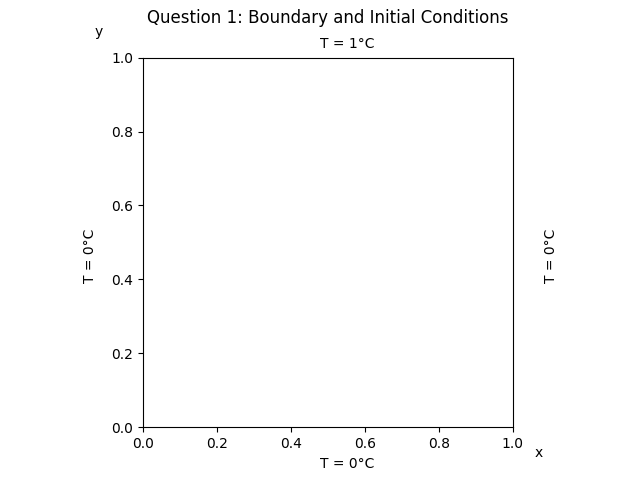
\includegraphics[width=0.5\textwidth]{figures/question1_initial}
		\caption{Boundary and initial conditions of question 1.}
		\label{question1_initial}
	\end{figure}
	
	There are numerous ways of tackling this problem numerically. In this homework assignment, the author attempted both the explicit and implicit methods. These methods have trade-offs which one should take into account when deciding which to employ. These trade-offs will be further discussed in various sections throughout the report, as well as in the \hyperref[discussion_section]{\emph{discussion} section}.
	
	\subsection{Explicit Method}
		Explicit methods involve directly computing the solution for the present state of a system from the (known) previous states. This is done by first employing the second order 5-point central differencing scheme for spacial discretisation and the first order forward differencing scheme for temporal discretisation to obtain \autoref{spacial_central_differencing} and \autoref{time_forward_differencing}. These expressions are then substituted into \autoref{heat_equation} to give
		\begin{equation}
			\frac{T_{i,j,k} - T_{i,j,k-1}}{\Delta t}
			=
			\frac{T_{i+1,j,k-1} - 2T_{i,j,k-1} + T_{i-1,j,k-1}}{(\Delta x)^2}
			+ 
			\frac{T_{i,j+1,k-1} - 2T_{i,j,k-1} + T_{i,j-1,k-1}}{(\Delta y)^2}
		\end{equation}
		
		Since $\Delta x = \Delta y$, the equation can be simplified to
		\begin{equation*}
			T_{i,j,k} = \lambda(T_{i-1,j,k-1} + T_{i+1,j,k-1} + T_{i,j-1,k-1} + T_{i,j+1,k-1} - 4*T_{i,j,k-1}) + T_{i,j,k-1}	
		\end{equation*}
		where $\lambda = \displaystyle{\frac{\Delta t}{(\Delta x)^2}}$. The temperature of each node within the boundary edges can thus be calculated directly from the temperature of nodes from the previous time step. The process can be repeated for every nodes on the plate for every time step increment until the temperature of the plate reaches steady state.
		
		The relative error in temperature, $\varepsilon_{temp}$, of each node at a given time step is calculated as
		\begin{equation}
			\varepsilon_{temp} = \frac{T_{i,j,k}-T_{i,j,k-1}}{T_{i,j,k}}\times 100\%
			\label{relative_error_temperature_formula}
		\end{equation}
		
		The temperature distribution across the plate is deemed to have reached steady state when the magnitude of the largest relative error of all the nodes across the plate is less than a prescribed percentage tolerance, $\varepsilon_s$
		\begin{equation*}
			\vert \varepsilon_{temp}\vert
			<
			\varepsilon_s
		\end{equation*}
		
		\cite{Scarborough1966} had shown that if the following criterion is met, we can be assured that the result obtained is correct to at least $n$ significant figures.
		\begin{equation}
			\varepsilon_s = (0.5 \times 10^{2-n})\%
			\label{scarborough_formula}
		\end{equation}
		
		For the purpose of this assignment, $n$ will be taken to be 4, which gives us $\varepsilon = 0.005\%$. Note that $\varepsilon_s$ will be referenced numerous times across this report as it is also used in the determination of the terminating condition of iterative methods later. 
		
		As mentioned earlier, different numerical methods have its upsides and downsides. One downside of the explicit method is that the size of the time step, $\Delta t$, is limited by a stringent criterion \citep{Chapra2010} in order for the system to be both convergent and stable. That criterion for this particular question is
		\begin{equation}
			\Delta t
			\leq
			\frac{(\Delta x)^2 + (\Delta y)^2}{8}
			\label{dt_criterion_explicit}
		\end{equation}
		
		Since $\Delta x = \Delta y = 0.04$ units, the value of $\Delta t$ used will be $0.0004$s. By using all the necessary parameters determined, the temperature distribution across the plate at various time ($t =$ 0.01s, 0.02s, 0.05s, 0.1s, \dots) is solved numerically and shown in \autoref{solution_1a_explicit}. Six different contour plots at various time are shown to depict the convergence of the result. Using the explicit method, the temperature distribution was found to reach steady state at $t=0.322$s (\autoref{solution_1a_explicit_ss}).
		
		\begin{figure}[H]
			\begin{subfigure}{0.5\textwidth}
				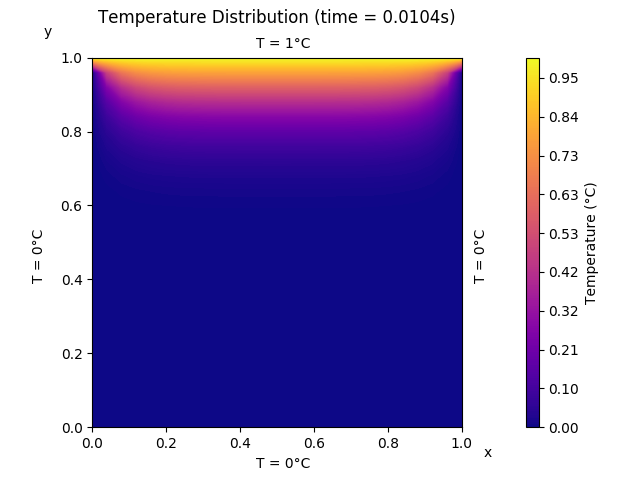
\includegraphics[width=\linewidth]{figures/1a_explicit/1)t=10ms.png}
				\caption{$t = 0.01$s}
			\end{subfigure}\hspace*{\fill}
			\begin{subfigure}{0.5\textwidth}
				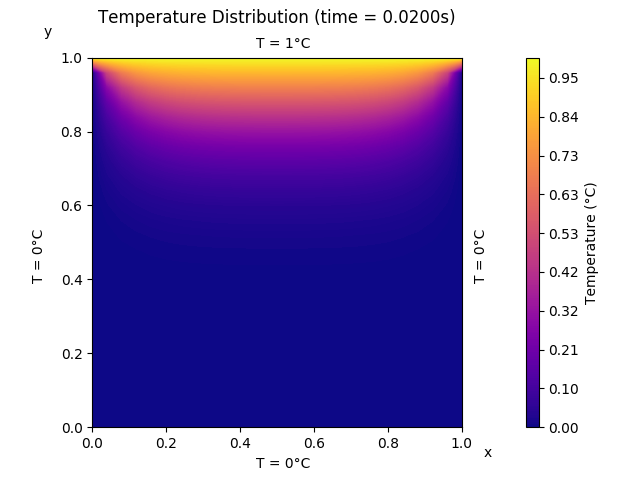
\includegraphics[width=\linewidth]{figures/1a_explicit/2)t=20ms.png}
				\caption{$t = 0.02$s}
			\end{subfigure}
			
			\medskip
			\begin{subfigure}{0.48\textwidth}
				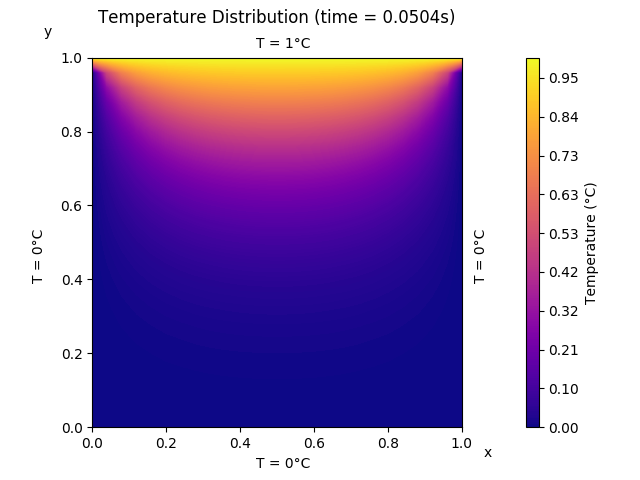
\includegraphics[width=\linewidth]{figures/1a_explicit/3)t=50ms.png}
				\caption{$t = 0.05$s}
			\end{subfigure}\hspace*{\fill}
			\begin{subfigure}{0.48\textwidth}
				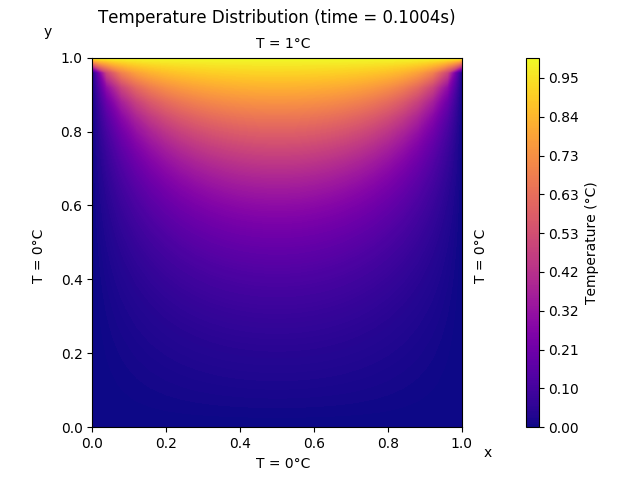
\includegraphics[width=\linewidth]{figures/1a_explicit/4)t=100ms.png}
				\caption{$t = 0.1$s}
			\end{subfigure}
			
			\medskip
			\begin{subfigure}{0.48\textwidth}
				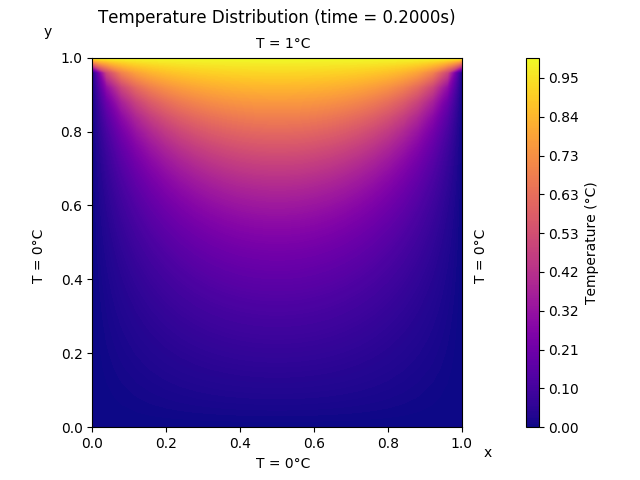
\includegraphics[width=\linewidth]{figures/1a_explicit/5)t=200ms.png}
				\caption{$t = 0.2$s}
			\end{subfigure}\hspace*{\fill}
			\begin{subfigure}{0.48\textwidth}
				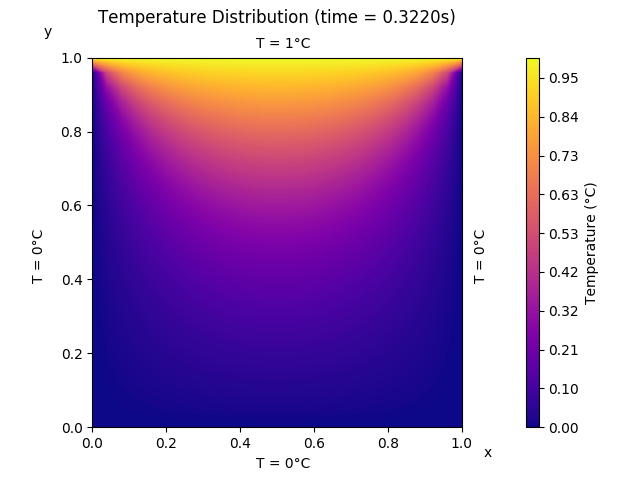
\includegraphics[width=\linewidth]{figures/1a_explicit/6)t=322ms(ss).png}
				\caption{$t = 0.322s \text{ (steady state)}$}
				\label{solution_1a_explicit_ss}
			\end{subfigure}
			
			\caption{Numerical solutions to question 1(a) using explicit method.} \label{solution_1a_explicit}
		\end{figure}
		
		The advantages of using explicit methods are that they are relatively easy to implement and they usually require less computation. Common sense would tell us that if the plate is divided into smaller partitions, we will be able to have a more `continuous' model of the plate and simulate the real situation better by reducing \textit{differencing error}. However, due to the criterion specified by \autoref{dt_criterion_explicit}, as the partition size decreases, the maximum allowable time step also decreases. If the time step used does not satisfy this criterion, truncation errors will magnify and the system becomes unstable.
		
		Problems that involve differential equations that require extremely small step size for explicit methods to be numerically stable are said to be \emph{stiff}. For such problems, implicit methods are used instead, this brings us to the next section.
		
	\subsection{Implicit Method}
		In this section, \textbf{question 1(a) is be solved again} using the implicit method. Implicit methods obtain solutions by solving equations involving both the current (unknown) state of the system as well as previous states. Implicit methods which often involve solving systems of equations (simultaneous equation) usually represented in the form of matrices. Due to this, implicit methods require higher computation and are generally harder to program or implement. However, implicit methods are much more stable. For stiff problems that would require impractically small time steps $\Delta t$ for explicit methods, implicit methods are often be able to produce solutions up to the same accuracy but with lower computational time by using larger time steps. The inherent stability of implicit methods makes them applicable to a much broader range of engineering problems.
	
		By employing the second order 5-point central differencing scheme for spacial discretisation and the first order backward differencing scheme for temporal discretisation, \autoref{spacial_central_differencing} and \autoref{time_backward_differencing} are obtained, which can be substituted into the \hyperref[heat_equation]{heat equation} (\autoref{heat_equation}) to give
		\begin{equation}
			\frac{T_{i,j,k} - T_{i,j,k-1}}{\Delta t}
			=
			\frac{T_{i+1,j,k} - 2T_{i,j,k} + T_{i-1,j,k}}{(\Delta x)^2}
			+ 
			\frac{T_{i,j+1,k} - 2T_{i,j,k} + T_{i,j-1,k}}{(\Delta y)^2}
			\label{heat_equation_differencing}
		\end{equation}
		
		Since $\Delta x = \Delta y$, the equation can be rearranged to give
		\begin{equation}
			(1 + 4\lambda)T_{i,j,k} - \lambda(T_{i+i,j,k} + T_{i-1,j,k} + T_{i,j+1,k} + T_{i,j-1,k})
			=
			T_{i,j,k-1}
			\label{1a_implicit_equation}
		\end{equation}
		where $\displaystyle{\lambda = \frac{\Delta t}{(\Delta x)^2}}$. This equation is for a particular node within the boundary edges of the plate. With $(M-1)(N-1)$ nodes within the edges of the plate, there will be $(M-1)(N-1)$ such equations and $(M-1)(N-1)$ unknowns to solve. This is typically done by constructing a linear matrix equation of the form $Ax=b$ and solving it, where $x$ is a matrix containing the temperatures of nodes across the plate, $A$ is a matrix of their coefficients and $b$ the constants. For the nodes next to the edges of the plate, some of the values of the terms on the left side of \autoref{1a_implicit_equation} are known from the given boundary conditions. These known values are thus shifted to the right side of the equation to be incorporated into matrix $b$. Matrix $b$ also contains the terms $T_{i,j,k-1}$ on the right side of \autoref{1a_implicit_equation}.
		
		There are various ways to solve the given problem implicitly. One way is by using \textit{direct methods}, for example the Gaussian elimination method. A more versatile and efficient way of solving larger scale problem is by using the \textit{iterative methods} (e.g. Jacobi method, Gauss-Seidel method) because the computation time taken is shorter for large matrices. For this homework assignment, the \emph{Jacobi's iterative method} is used. The author implemented the Jacobi's method in Python to solve the plate's temperature distribution numerically.
		\lstinputlisting[language=Python]{content/jacobi.py}
		
		In order to test for the correct functioning of this implementation, the Jacobi's method implemented is tested by comparing its output solutions to simple linear matrix equations with solutions calculated by hand. The computed results for larger linear matrix equations were also tested by comparing them to that of \href{https://docs.scipy.org/doc/numpy/reference/generated/numpy.linalg.solve.html}{SciPy's linear equation matrix solver}.
		
		In order to make a comparison in the time taken to reach steady state with that obtained from the explicit method, the time step used is set to $\Delta t=0.0004$s. The relative error, $\varepsilon_a$, of each node on the plate at each iteration is calculated as
		\begin{equation}
			\varepsilon_a = \frac{x_n - x_{n-1}}{x_n}\times 100\%
			\label{relative_error_formula}
		\end{equation}
		where $n$ is the number of iterations.
		
		For the iterations at each time step increment, the computed result is deemed accurate enough for iteration to stop when the magnitudes of the relative errors of all nodes on the plate is less than the prescribed percentage tolerance, $\varepsilon_s = 0.005\%$ as calculated from \autoref{scarborough_formula}. The condition used to determine steady state is the same as that in the previous section, whereby the relative error in temperature is calculated using \autoref{relative_error_temperature_formula} and ensuring all the nodes on the plate satisfy the condition of $\vert\varepsilon_{temp}\vert < \varepsilon_s$. The numerical solution using the iterative method is shown in \autoref{solution_1a_implicit}. Using the Jacobi's iteration method, the temperature distribution was found to reach steady state at $t=0.324$s (\autoref{solution_1a_implicit_ss}), which is very close to that computed using the explicit method (\autoref{solution_1a_explicit_ss}).
		
		\begin{figure}[H]
			\begin{subfigure}{0.5\textwidth}
				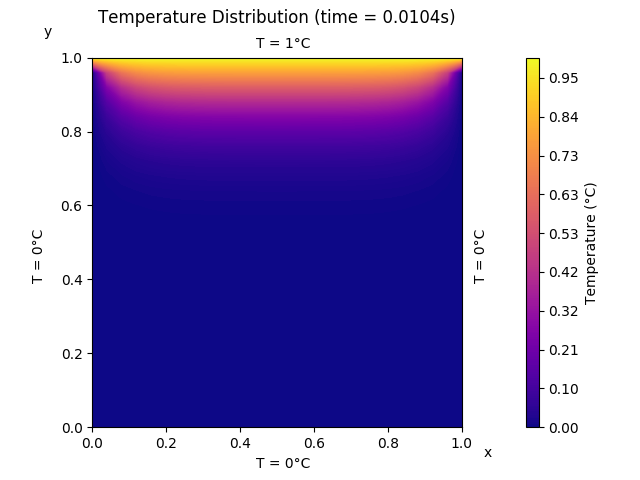
\includegraphics[width=\linewidth]{figures/1a_implicit/1)t=10ms.png}
				\caption{$t = 0.01$s}
			\end{subfigure}\hspace*{\fill}
			\begin{subfigure}{0.5\textwidth}
				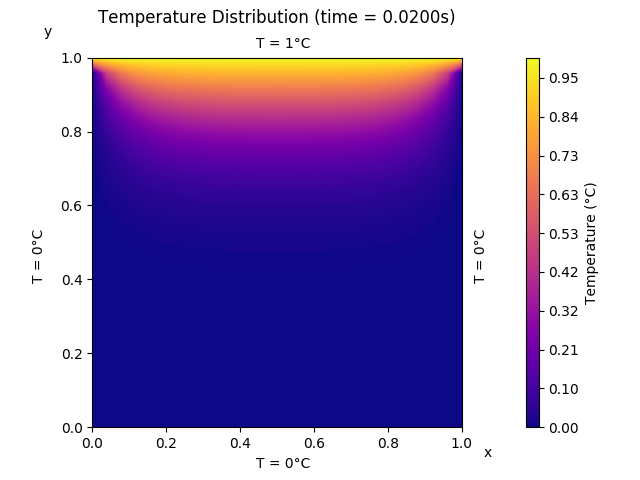
\includegraphics[width=\linewidth]{figures/1a_implicit/2)t=20ms.png}
				\caption{$t = 0.02$s}
			\end{subfigure}
			
			\medskip
			\begin{subfigure}{0.48\textwidth}
				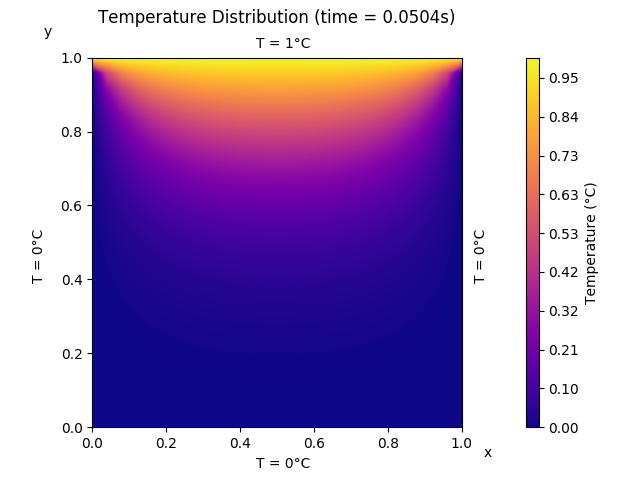
\includegraphics[width=\linewidth]{figures/1a_implicit/3)t=50ms.png}
				\caption{$t = 0.05$s}
			\end{subfigure}\hspace*{\fill}
			\begin{subfigure}{0.48\textwidth}
				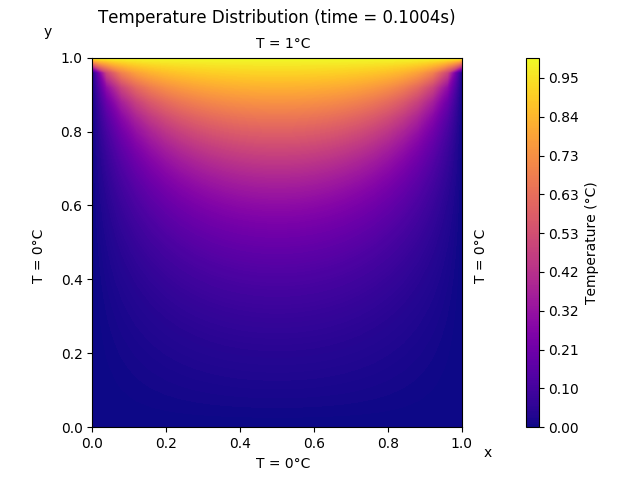
\includegraphics[width=\linewidth]{figures/1a_implicit/4)t=100ms.png}
				\caption{$t = 0.1$s}
			\end{subfigure}
			
			\medskip
			\begin{subfigure}{0.48\textwidth}
				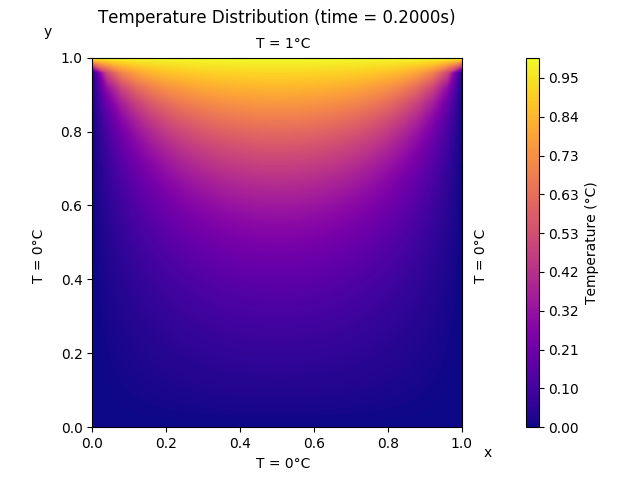
\includegraphics[width=\linewidth]{figures/1a_implicit/5)t=200ms.png}
				\caption{$t = 0.2$s}
			\end{subfigure}\hspace*{\fill}
			\begin{subfigure}{0.48\textwidth}
				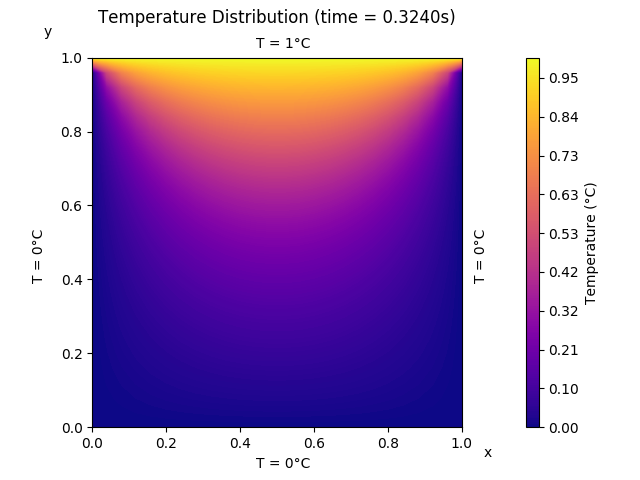
\includegraphics[width=\linewidth]{figures/1a_implicit/6)t=324ms(ss).png}
				\caption{$t = 0.324s \text{ (steady state)}$}
				\label{solution_1a_implicit_ss}
			\end{subfigure}
			
			\caption{Numerical solutions to question 1(a) using Jacobi's iterative method.} \label{solution_1a_implicit}
		\end{figure}
		
		The author also obtained numerical solutions by using time steps $\Delta t$ of different sizes to observe the effects on the numerical solutions. Some of the solutions obtained at selected time step sizes are shown in \autoref{solution_1a_implicit_dt_varies}. It was discovered that the implicit iterative method remains stable regardless of the size of time step, producing identical contour plots. The rate of convergence is also found to increases as the size of time step increases. However, at larger time steps, the accuracy of the calculated total time to reach steady state decreases. This may be attributed to the increase in the accumulation of truncation error in the increased amount of computation. It was also found that as the number of partitions increases, the computation time taken increases. This makes sense as more computation is required for operation such as matrix manipulation and inversion as the size of the matrices increases.
		\begin{figure}[H]
			\begin{subfigure}{0.5\textwidth}
				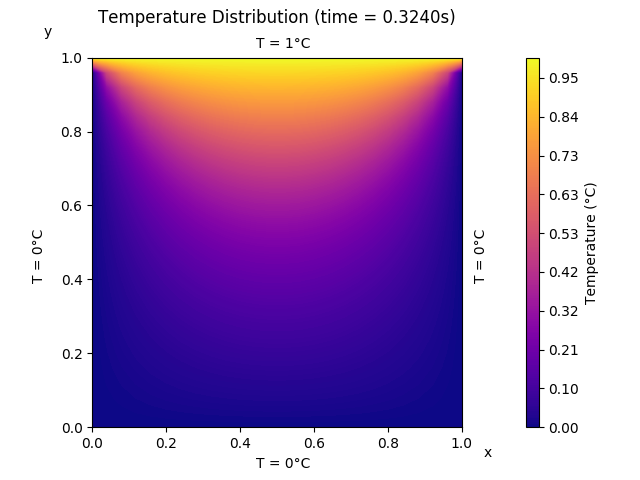
\includegraphics[width=\linewidth]{figures/1a_implicit_dt_varies/1)dt=400ns.png}
				\caption{$\Delta t = 0.0004$s}
			\end{subfigure}\hspace*{\fill}
			\begin{subfigure}{0.5\textwidth}
				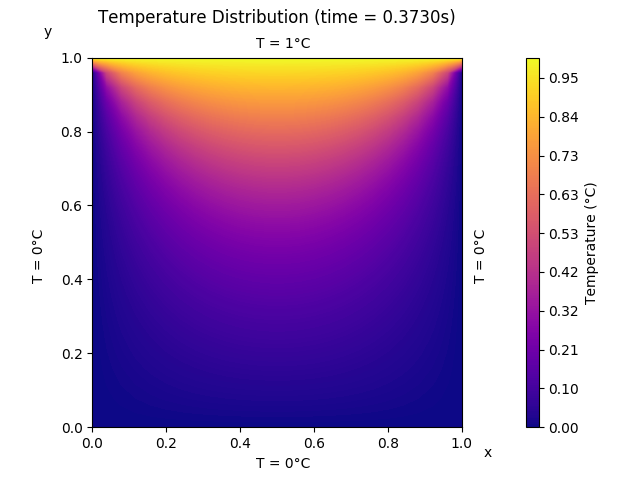
\includegraphics[width=\linewidth]{figures/1a_implicit_dt_varies/2)dt=1000ns.png}
				\caption{$\Delta t = 0.001$s}
			\end{subfigure}
			
			\medskip
			\begin{subfigure}{0.48\textwidth}
				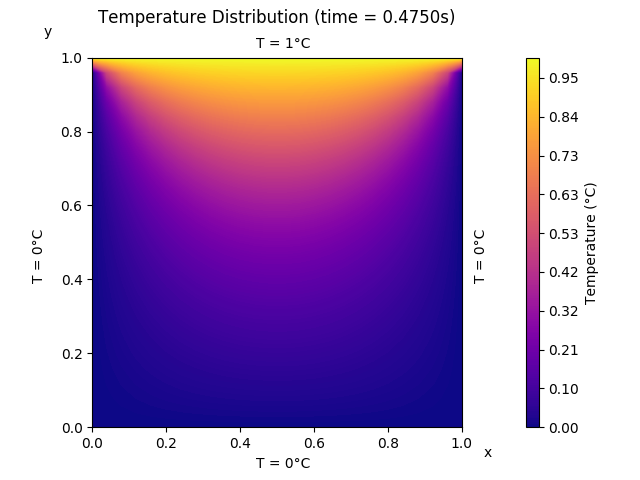
\includegraphics[width=\linewidth]{figures/1a_implicit_dt_varies/3)dt=5000ns.png}
				\caption{$\Delta t = 0.005$s}
			\end{subfigure}\hspace*{\fill}
			\begin{subfigure}{0.48\textwidth}
				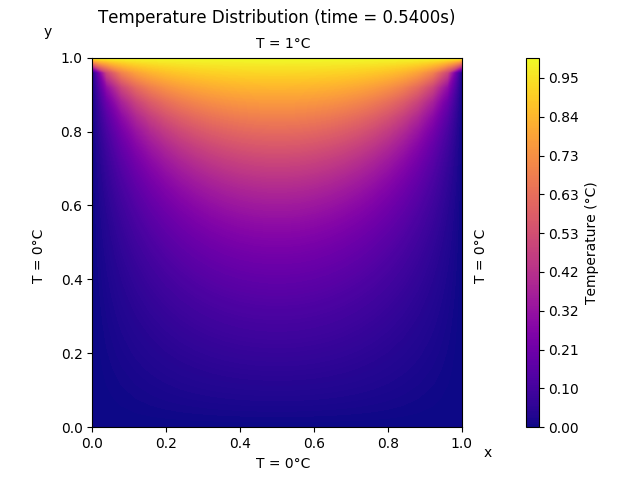
\includegraphics[width=\linewidth]{figures/1a_implicit_dt_varies/4)dt=10000ns.png}
				\caption{$\Delta t = 0.01$s}
			\end{subfigure}
			
			\caption{Effect of varying $\Delta t$ on numerical solutions using implicit method.} \label{solution_1a_implicit_dt_varies}
		\end{figure}
	
\section{Question 1(b) -- Dirichlet Boundary Conditions (Steady State)}
	In question 1(b), the boundary conditions are identical to that of part(a). This section requires that, instead of solving for the steady state by marching through time, the steady state can be solved directly by letting $\displaystyle{\frac{\partial T}{\partial t} = 0}$. Thus, from the \hyperref[heat_equation]{heat equation} (\autoref{heat_equation}) we obtain the Laplace equation
	\begin{equation*}
		0 = \frac{\partial^2 T}{\partial x^2} + \frac{\partial^2 T}{\partial y^2}
	\end{equation*}
	
	By employing the second order 5-point central differencing scheme for spacial discretisation to obtain \autoref{spacial_central_differencing} and substituting it into the Laplace equation, we now have
	\begin{equation}
		0 =
		\frac{T_{i+1,j,k} - 2T_{i,j,k} + T_{i-1,j,k}}{(\Delta x)^2}
		+ 
		\frac{T_{i,j+1,k} - 2T_{i,j,k} + T_{i,j-1,k}}{(\Delta y)^2}
		\label{laplace_equation_2}
	\end{equation}

	Since $\Delta x = \Delta y$, the Laplace equation can be simplified to
	\begin{equation*}
		T_{i+1,j,k} + T_{i-1,j,k}
		+ T_{i,j+1,k} + T_{i,j-1,k}
		- 4T_{i,j,k} = 0
		\label{1b_implicit_equation}
	\end{equation*}
	
	Similar to how the linear matrix equation is constructed in part(a), the system of $(M-1)(N-1)$ number of equations for each node in the form of \autoref{1b_implicit_equation} can be represented by a linear matrix equation of the form $Ax=b$, where $x$ is a matrix containing the temperatures of all the nodes to solve, $A$ is a matrix of their coefficients and matrix $b$ incorporates the known values of some the terms on the left side of \autoref{1b_implicit_equation} from the boundary condition.
	
	The implementation of the Jacobi's iterative method for part(a) can be reused for this section. To be consistent, the same iteration termination condition as the previous section is used, whereby the relative error of each iteration is calculated using \autoref{relative_error_formula} and compared with $\vert \varepsilon_s \vert < 0.005\%$, stopping the iteration when $\vert \varepsilon_a \vert < \varepsilon_s$.
	
	The steady state condition used for the temperature distribution is also kept consistent with that of part(a), whereby the relative error in temperature is calculated using \autoref{relative_error_temperature_formula} and steady state is reached when all nodes on the plate satisfy the condition of $\vert\varepsilon_{temp}\vert < \varepsilon_s$. With this, the linear matrix equation is solved and the result is shown in \autoref{solution_1b_implicit_ss}.
	\begin{figure}[H]
		\centering
		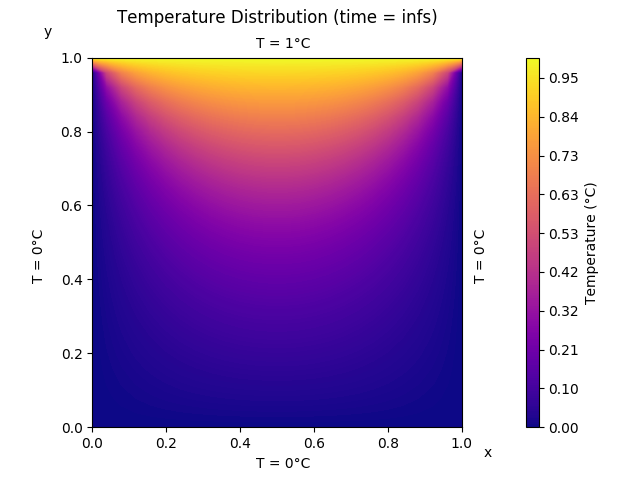
\includegraphics[width=0.5\textwidth]{figures/1b/t=inf}
		\caption{Steady state solution to question 1(b) using Jacobi's iterative method.}
		\label{solution_1b_implicit_ss}
	\end{figure}
	
	The contour plot obtained for steady state is very identical to that in part(a). This is a good sign that the solution is likely to be correct. Compared to the methods in part(a), if the goal is to obtain the temperature distribution contour without needing to know the time elapsed at steady state, then this method (without marching through time) is more efficient as it takes much less iteration and thus computation time.
	
\section{Question 2 -- Neumann Boundary Condition}
	Question 2 imposes the Neumann boundary condition along the right edge of the plate. In this case, the right edge of the plate is insulated. This means that the heat flux is 0 across the right edge of the plate
	$$ \frac{\partial T}{\partial x} = 0 $$	
	The same Dirichlet boundary conditions apply to the remaining three edges of the plate, with the top edge maintained at \degC{1} and the remaining two edges at \degC{0} as shown below.
	\begin{figure}[H]
		\centering
		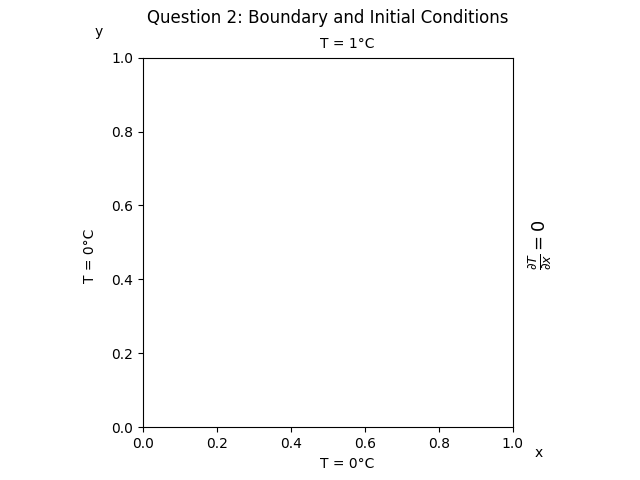
\includegraphics[width=0.5\textwidth]{figures/question2_initial}
		\caption{Boundary and initial conditions of question 2.}
		\label{question2_initial}
	\end{figure}
	
	Due to the Neumann boundary condition, the temperatures of the nodes along the right edge of the plate are now unknowns. There are different ways to tackle this problem. In order to reuse the functions and methods implemented in solving question 1, the method used for this homework assignment is to express the temperature of the nodes along the right edge of the plate in terms of the boundary condition derivative.
	
	For each nodes along the right edge of the plate $(M,j)$, by using the first order central differencing scheme, the flux in the $x$-direction can be represented as
	\begin{equation*}
		\frac{\partial T}{\partial x}
		\cong
		\frac{T_{M,j} - T_{M+1,j}}{2\Delta x}
		%\label{neumann_boundary_condition_central_differencing}
	\end{equation*}
	where $(M+1,j)$ represents imaginary points outside the right edge of the plate. We can then solve for
	\begin{equation*}
		T_{M+1,j} =
		T_{M,j} + 2\Delta x \frac{\partial T}{\partial x}
	\end{equation*}
	Substituting this expression into \autoref{heat_equation_differencing} and rearranging gives
	\begin{equation}
		(1 + 4 \lambda) T_{i,j,k}
		- \lambda(T_{i-1,j,k} + T_{i,j-1,k} + 2T_{i,j+1,k})
		=
		T_{i,j,k-1}
		\label{2_implicit_equation}
	\end{equation}
	where $\displaystyle{\lambda = \frac{\Delta t}{(\Delta x)^2}}$. Unlike question 1, there are now $(M)(N-1)$ number of unknowns and $(M)(N-1)$ number of equations in the form of \autoref{2_implicit_equation} to solve. Using this system of simultaneous equations, we can form a linear matrix equation in the form of $Ax=b$, where $x$ is a matrix containing the temperatures of the unknowns to solve, $A$ is a matrix of their coefficients, and matrix $b$ contains the temperatures of $T_{i,j,k-1}$ as well as the known values on the left side of \autoref{2_implicit_equation} from the boundary conditions.
	
	To be consistent with the previous sections, the size of the time step $\Delta t$ used is $0.0004$s. The condition used to terminate the iteration process at each time step increment and the steady state condition used are also the same as that described in question 1, whereby the relative errors of each iterations and the relative errors in temperature distribution at each time steps are calculated and compared to the prescribed percentage tolerance $\varepsilon_s = 0.005\%$, stopping when $\vert \varepsilon_{temp} \vert < \varepsilon_s$ and $\vert \varepsilon_a \vert < \varepsilon_s$ respectively. With the same initial conditions as before ($T=$\degC{0} at $t=0$s for the whole domain), the numerical solution obtained is presented in \autoref{solution_2}.
	\begin{figure}[H]
		\begin{subfigure}{0.5\textwidth}
			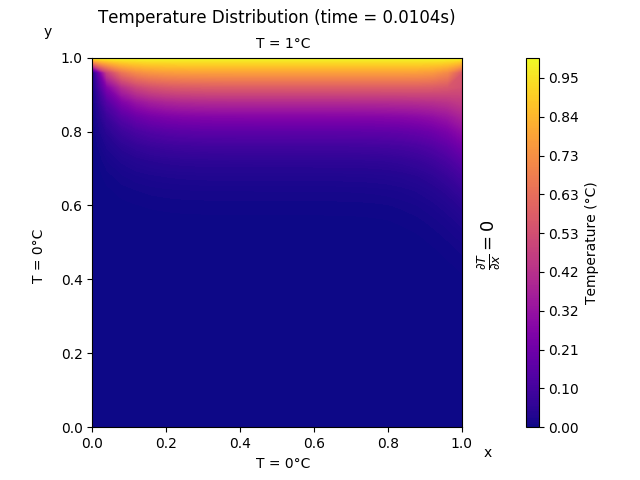
\includegraphics[width=\linewidth]{figures/2/1)t=10ms.png}
			\caption{$t = 0.01$s}
		\end{subfigure}\hspace*{\fill}
		\begin{subfigure}{0.5\textwidth}
			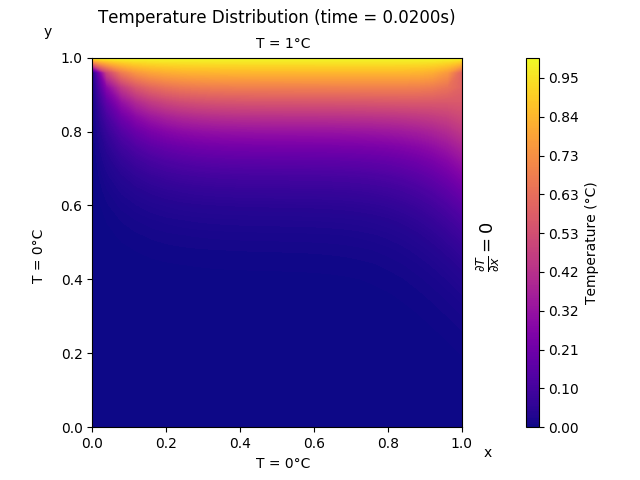
\includegraphics[width=\linewidth]{figures/2/2)t=20ms.png}
			\caption{$t = 0.02$s}
		\end{subfigure}
		
		\medskip
		\begin{subfigure}{0.48\textwidth}
			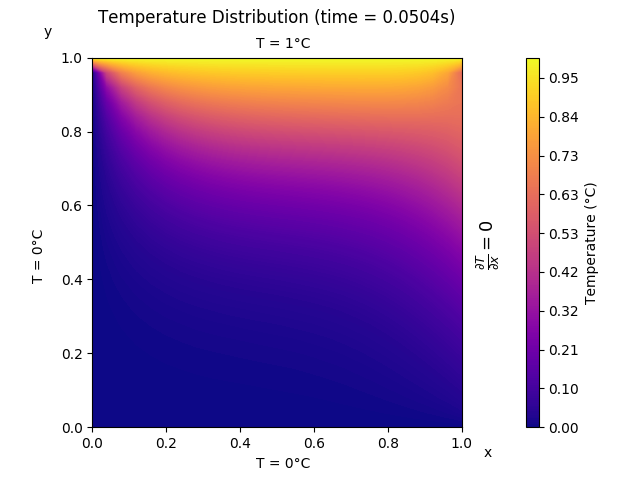
\includegraphics[width=\linewidth]{figures/2/3)t=50ms.png}
			\caption{$t = 0.05$s}
		\end{subfigure}\hspace*{\fill}
		\begin{subfigure}{0.48\textwidth}
			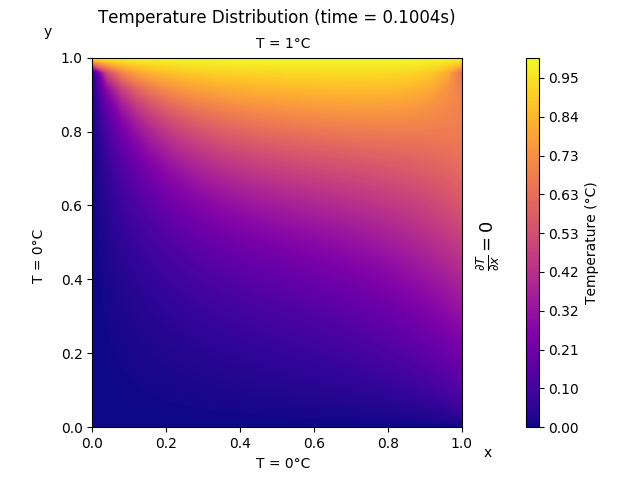
\includegraphics[width=\linewidth]{figures/2/4)t=100ms.png}
			\caption{$t = 0.1$s}
		\end{subfigure}
		
		\medskip
		\begin{subfigure}{0.48\textwidth}
			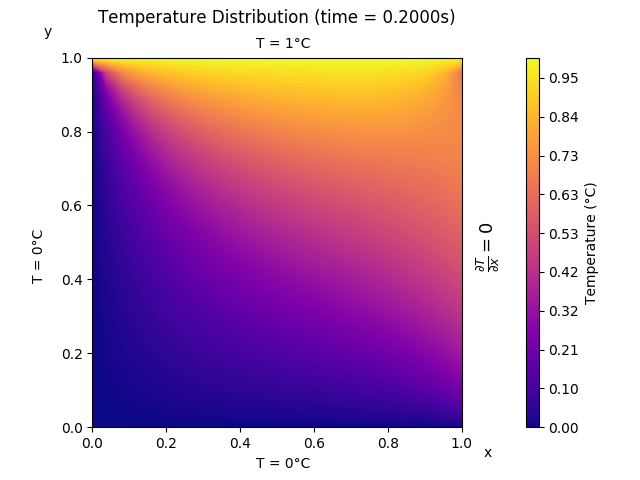
\includegraphics[width=\linewidth]{figures/2/5)t=200ms.png}
			\caption{$t = 0.2$s}
		\end{subfigure}\hspace*{\fill}
		\begin{subfigure}{0.48\textwidth}
			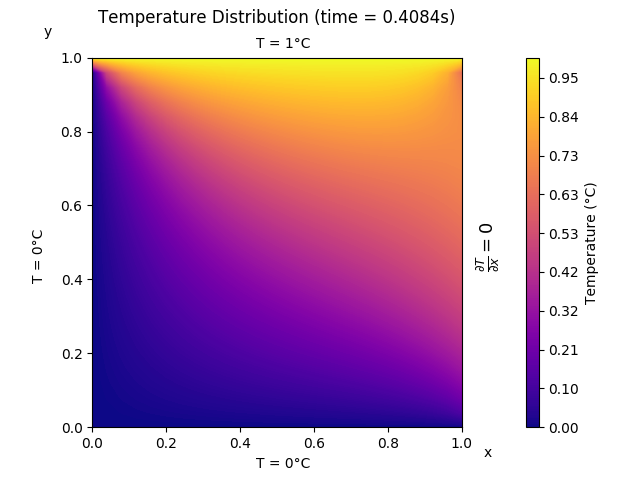
\includegraphics[width=\linewidth]{figures/2/6)t=408ms(ss).png}
			\caption{$t = 0.4084s \text{ (steady state)}$}
			\label{solution_2_ss}
		\end{subfigure}
		
		\caption{Numerical solutions to question 2 using implicit iterative method.} \label{solution_2}
	\end{figure}
	
	The numerical solutions obtained are consistent with the physics of heat transfer. Compared to solutions of question 1 (\autoref{question1_initial}), the part of the plate along the right edge is at higher temperature. This makes sense because heat cannot `escape' via the right edge of the plate and thus accumulates more in that region, and the heat flux is deflected downwards and leftwards along the right edge. Note that the darker spot at the top-right corner of the plate is not a bug, it is due to the limitation of finite partitioning of the plate $(M=N=25)$.
	
\section{Discussions}
\label{discussion_section}
	This section will further discuss the process of testing for correctness of the numerical solutions obtained and the trade-offs between explicit and implicit methods. Limitations of the methods used in this homework assignment will also be discussed and possible improvements recommended.
	
	\subsection{Correctness of Results}
		In numerical methods, it can sometimes be tricky to determine whether a solution is correct or not. While working on the homework assignment, there were numerous occurrences when solutions look fine at first sight but was found to be `buggy' or erroneous upon further scrutiny.
	
		\textbf{Plotting and visualisation} is one of the most useful ways of checking numerical solutions. Contour plots are used for the purpose of this assignment. The contour plot is also animated to observe the transient process for detection of errors in the transient phase.
		
		\textbf{Programming style} also affects the ease of testing programs. By using appropriate comments in the source code, encapsulating frequently used code into modular and generalised functions, implementations may become less error-prone and testing can be made much easier.
		
		\textbf{Testing with small samples} is another very useful way to check the correct functionality of programs. An example that is appropriate for this assignment problem would be to set $M=N=4$, whereby the systems of equation is small enough to be calculated by hand which can then be used to compare to the output of the program to ensure correct functionality. This method had helped the author to locate and `catch' numerous `bugs' while working on the homework assignment.
		
		\textbf{Comparison between solutions of different methods} will also indicate the correctness of programs or methods. This is done in question 1(a) by comparing the results obtained with the explicit method and the implicit iterative method. The steady state solution obtained in question 1(a) is also compared to that of question 1(b).
		
		\textbf{Understanding the problem well} is also very important for an engineer to formulate expectations which can be used as the basis of comparison with the numerical solutions obtained. This can be seen in the discussion of question 2 regarding the consistency of the numerical solution with the physics of heat transfer. The numerical methods are also employed with varying parameters (e.g. size of time step, number of partitions) and the results are observed and compared to expectations based on the physics of heat transfer.
		
	\subsection{Trade-Offs: Explicit vs Implicit Method}
		This section summarises the trade-offs between different numerical methods used in this homework assignment, namely the explicit and implicit methods.
		
		\textbf{Explicit methods} require less computation and are easier to implement and program. However, depending on the problem, it can sometimes be difficult to compute the state of a system solely based on its previous state. Also, due to the limiting criterion for the maximum allowable time step $\Delta t$ as described by \autoref{dt_criterion_explicit}, the use of explicit methods to solve \textit{stiff} equations usually requires impractically small time steps to remain convergent and stable.
		
		It is for these reasons that \textbf{implicit methods} are more commonly used in real world engineering problems. To achieve a given accuracy in cases where problem are \emph{stiff}, implicit methods are able to produce results in a shorter amount of time as they are stable even when larger time steps are used. The stability of implicit methods allows it to be applied to a much broader range of problem compared to explicit methods. The downsides of implicit methods are that they are usually harder to program and require higher computation.
		
	\subsection{Limitations and Possible Improvements}
		As ME3291 is an introductory course to numerical methods, the author merely learned about the basics of numerical methods which limits the author's ability to solve the assignment problem in the most efficient way possible. This section will outline the various improvements that can be made to improve the efficiency or accuracy of the numerical methods.
		
		First of all, more advanced numerical methods such as the \emph{Alternating Direction Implicit (ADI) method} can be used to solve the problem more efficiently. Furthermore, methods such as the successive over-relaxation method can be used with the Gauss-Seidel method to hasten convergence of iterative methods. Solving the system more efficiently means smaller time steps or larger matrices can be used, which improves the simulation or numerical solution.
		
		Finally, readers should be reminded that the very first assumption made in this homework assignment in letting the thermal diffusivity $\alpha$ in the \hyperref[ori_heat_equation]{heat equation} (\autoref{ori_heat_equation}) to be 1 m$^2/$s had already posed limitations to the simulation results in simulating real world situations (even though it is a necessary assumption because the plate's material is not specified). Even the most (thermally) conductive material such as gold and pure silver have thermal diffusivity values in the order of magnitude of $10^{-4}$ m$^2$/s \citep{Brown1958}. When the thermal diffusivity of pure silver ($\alpha = 1.6563\times 10^{-4}$ m$^2/$s) is used by the author with time steps of size $\Delta t = 0.1$s, the total time taken for the temperature distribution to reach steady state was a whopping 16.8 minutes (rather than mere seconds) as shown in \autoref{pure_silver_simulation}.
		\begin{figure}[H]
			\centering
			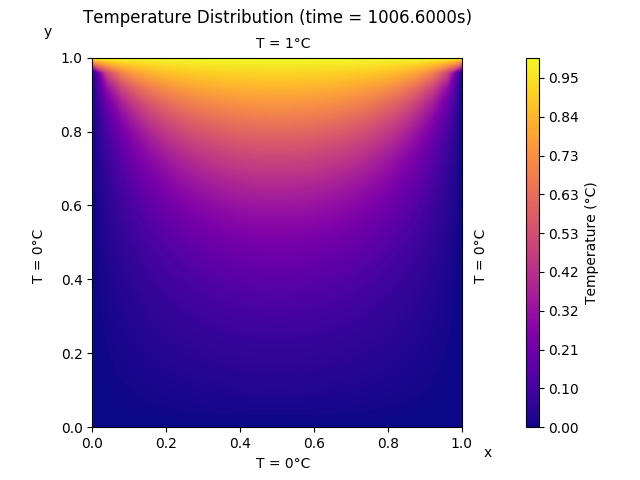
\includegraphics[width=0.5\textwidth]{figures/pure_silver}
			\caption{Steady state temperature distribution of pure silver plate.}
			\label{pure_silver_simulation}
		\end{figure}
		
\section{Conclusion}
	This assignment had helped the author greatly in learning and appreciating the basic concepts of numerical methods. Extensive experimentation was done in programming and testing the numerical methods. Considering the agreement of the numerical solutions with the physics of heat transfer as well as the agreement between the results produced by different numerical methods, the author is confident that the numerical solutions obtained are satisfactory in simulating heat transfer across a square plate.

%%%%%%%%%%%%%%%%%%%%%%%%%%%%%%%%%%%%%%%%%%%%%%%%%%%%%%%%%%%
%\newpage
\bibliographystyle{abbrvnat}
%\bibliographystyle{plainnat}
\bibliography{literature/me3291_reference_list}

%%%%%%%%%%%%%%%%%%%%%%%%%%%%%%%%%%%%%%%%%%%%%%%%%%%%%%%%%%%
\newpage
\begin{appendix}
\section{Program Code}
	\label{complete_code}
	\lstinputlisting[language=Python]{content/complete_code.py}
\end{appendix}

\end{document}